\documentclass[dvipdfmx,a4paper,11pt]{jsarticle}
\usepackage[dvipdfmx]{graphicx}
\usepackage{amsmath,amssymb}
\usepackage{geometry}
\usepackage{booktabs,array}
\usepackage{tikz}
\usepackage{jikkenTitle}
\geometry{left=25mm,right=25mm,top=30mm,bottom=30mm}
\renewcommand{\arraystretch}{1.15}
\begin{document}
\begin{jikkenTitle}
  \gakunen{8}{4}
  \numTitle{1}{制御系実験}
  \subTitle{テーマ一 QUBE-Servo の基本及びフィルタリング、モデリング手法}
  \jikkenbi{}
  \kyoudou{}
  \preYoteibi{}\preTeishutsubi{}\repYoteibi{}\repTeishutsubi{}
  \hanNumberName{9}{4326}{中野光喜}
\end{jikkenTitle}

\section*{テーマ一 QUBE-Servo の基本及びフィルタリング、モデリング手法}
\addcontentsline{toc}{section}{テーマ一 QUBE-Servo の基本及びフィルタリング、モデリング手法}
\section{目的}
QUBE-Servo と LabVIEW の接続を通して，直流モータの駆動とエンコーダによる回転角の計測方法を身につける。次に，角度信号から回転速度を求め，ローパスフィルタによって計測ノイズを抑える方法とその応答への影響を理解する。さらに，ステップ応答から一次遅れモデルのゲインと時定数を同定し，計測値とモデル出力を比較してモデルの妥当性を調べる。最後に，モータの電気・機械特性から運動方程式を組み立て，物理パラメータに基づくモデルを実測応答と比較する。

\section{関連知識}
\subsection{LabVIEW と QUBE-Servo}
LabVIEW は，計測・制御処理をブロックダイアグラムで構成する開発環境である。作成した仮想計測器（VI）のフロントパネルから入力値を変更し，出力波形を観察できる。本実験では Quanser Rapid Control Prototyping Toolkit（RCP）の HIL Initialize，HIL Read，HIL Write を介して myRIO に接続した QUBE-Servo を操作する。QUBE-Servo は PWM アンプで駆動するブラシ付き直流モータ，回転角を測るエンコーダ，ハブおよび慣性ディスクからなる。制御・シミュレーションループの刻み幅を $0.002\,\mathrm{s}$ とすると，サンプリング周波数は $500\,\mathrm{Hz}$ になる\cite{manual}。

\subsection{DC モータとエンコーダ}
直流モータでは，電機子電流がトルクを生み，印加電圧を上げると一般に定常回転速度が上がる。回転角 $\theta_m$ と角速度 $\omega_m$ は $\omega_m=d\theta_m/dt$ の関係にある。一定電圧の下で角速度が定常値に近づけば，角度は時間に対してほぼ直線的に増加する。ただし，負荷や摩擦が変わると同じ電圧でも回転速度は変化する。

本装置のインクリメンタル形エンコーダは $512$ ラインを持ち，直交デコーダで4逓倍するため，分解能は $2048$ カウント/回転である\cite{manual}。したがってカウント値 $n$ からの角度換算は
\begin{equation}
 \theta_m[^{\circ}]=\frac{360}{2048}n=0.17578125n,\qquad
 \theta_m[\mathrm{rad}]=\frac{2\pi}{2048}n=\frac{\pi}{1024}n
 \label{eq:encoder}
\end{equation}
となる。エンコーダは起動位置からの相対角を出力する。myRIO のカウンタは16 bitであるため，カウント値を連続的な角度に直す際には $65536$ カウントでの折り返しを補正する。

\subsection{ローパスフィルタ}
一次ローパスフィルタは低周波成分を通し，高周波成分を減衰させる。伝達関数は
\begin{equation}
 G_f(s)=\frac{\omega_f}{s+\omega_f}
 \label{eq:lpf}
\end{equation}
であり，$\omega_f$ はカットオフ角周波数 $[\mathrm{rad/s}]$ である。周波数 $[\mathrm{Hz}]$ では $f_f=\omega_f/(2\pi)$ と表す。$\omega_f=50\,\mathrm{rad/s}$ は約 $7.96\,\mathrm{Hz}$ に相当する。エンコーダの角度はカウント単位で階段状に変わるため，そのまま微分すると変化点で速度信号が大きく揺らぐ。式\eqref{eq:lpf}を微分後の信号に適用すると揺らぎを抑えられるが，カットオフ周波数を低くしすぎると応答の遅れが増す。

\subsection{一次遅れ系の伝達関数とステップ応答}
入力 $u$，出力 $y$ の一次遅れ系は，ゲイン $K$，時定数 $\tau$ を用いて
\begin{equation}
 G(s)=\frac{Y(s)}{U(s)}=\frac{K}{\tau s+1}
 \label{eq:first}
\end{equation}
と書ける。図\ref{fig:bump}のように時刻 $t_0$ に入力を $u_{\min}$ から $u_{\max}$ へ変えたとき，$\Delta u=u_{\max}-u_{\min}$，$\Delta y=y_{\mathrm{ss}}-y_0$ とすると
\begin{equation}
 K=\frac{\Delta y}{\Delta u},\qquad
 y(t_1)=y_0+0.632\Delta y,\qquad
 \tau=t_1-t_0
 \label{eq:bump}
\end{equation}
である。初期値を $\omega_m(t_0)$，ステップ電圧の変化量を $A_v$ とすると，$t\geq t_0$ の角速度応答は
\begin{equation}
 \omega_m(t)=\omega_m(t_0)+KA_v\left(1-e^{-(t-t_0)/\tau}\right)
 \label{eq:step}
\end{equation}
となる\cite{manual}。$K$ は定常速度の変化量，$\tau$ は最終変化量の約63.2\%に到達するまでの時間から求める。
\begin{figure}[htbp]\centering
\begin{tikzpicture}[x=1cm,y=0.75cm,>=stealth]
 \draw[->] (0,0)--(8,0) node[right]{$t$};
 \draw[->] (0,0)--(0,4.2) node[above]{信号};
 \draw[thick,blue] (0,0.45)--(1.5,0.45)--(1.5,1.35)--(7.5,1.35);
 \node[blue,anchor=west] at (6.3,1.55) {$u(t)$};
 \draw[thick,red,domain=1.5:7.4,samples=100] plot (\x,{0.55+2.65*(1-exp(-(\x-1.5)/1.25))});
 \draw[red,dashed] (0,3.2)--(7.5,3.2) node[right]{$y_{\mathrm{ss}}$};
 \draw[dashed] (1.5,0)--(1.5,3.5);
 \draw[dashed] (2.75,0)--(2.75,2.25);
 \node[below] at (1.5,0) {$t_0$};\node[below] at (2.75,0) {$t_1$};
 \node[red,anchor=west] at (5.2,2.7) {$y(t)$};
 \node[left] at (0,0.55) {$y_0$};
\end{tikzpicture}
\caption{一次遅れ系のステップ入力と応答（指導書の図3.1を基に作図）}\label{fig:bump}
\end{figure}

\subsection{QUBE-Servo の数学モデル及び各パラメータ}
図\ref{fig:motor}のように，モータの電機子回路には巻線抵抗 $R_m$，インダクタンス $L_m$，逆起電力 $e_b$ がある。逆起電力定数を $k_m$ とすると $e_b=k_m\omega_m$ であり，キルヒホッフの法則から
\begin{equation}
 v_m=R_m i_m+L_m\frac{di_m}{dt}+k_m\omega_m
 \label{eq:electrical}
\end{equation}
を得る。$L_m$ の影響を無視する近似では
\begin{equation}
 i_m=\frac{v_m-k_m\omega_m}{R_m}
 \label{eq:current}
\end{equation}
となる。トルク定数を $k_t$，等価慣性モーメントを $J_{\mathrm{eq}}$ とすれば，摩擦を無視した回転運動方程式は
\begin{equation}
 J_{\mathrm{eq}}\frac{d\omega_m}{dt}=\tau_m=k_t i_m
 \label{eq:motion}
\end{equation}
である。質量 $m$，半径 $r$ の一様な円板の慣性モーメントは $J=mr^2/2$ であり，$J_{\mathrm{eq}}=J_m+J_h+J_d$，$J_d=m_dr_d^2/2$ として求める。表\ref{tab:params}の値では $J_d=1.63\times10^{-5}\,\mathrm{kg\,m^2}$，$J_{\mathrm{eq}}\simeq2.09\times10^{-5}\,\mathrm{kg\,m^2}$ となる。式\eqref{eq:current}と式\eqref{eq:motion}を連結すれば，印加電圧から回転速度までを計算するモデルになる。
\begin{figure}[htbp]\centering
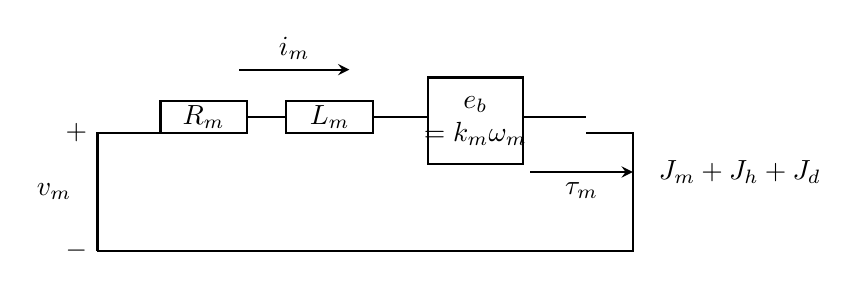
\begin{tikzpicture}[>=stealth,thick]
 \draw (0,0)--(0,1.5)--(0.8,1.5);
 \draw (0,0)--(6.8,0)--(6.8,1.5)--(6.2,1.5);
 \draw (0.8,1.5) rectangle (1.9,1.9) node[pos=.5]{$R_m$};
 \draw (1.9,1.7)--(2.4,1.7);
 \draw (2.4,1.5) rectangle (3.5,1.9) node[pos=.5]{$L_m$};
 \draw (3.5,1.7)--(4.2,1.7);
 \draw (4.2,1.1) rectangle (5.4,2.2) node[pos=.5,align=center]{$e_b$\\$=k_m\omega_m$};
 \draw (5.4,1.7)--(6.2,1.7);
 \draw[->] (1.8,2.3)--(3.2,2.3) node[midway,above]{$i_m$};
 \node[left] at (0,1.5) {$+$};\node[left] at (0,0) {$-$};
 \node[left] at (-0.2,0.75) {$v_m$};
 \draw[->] (5.5,1.0)--(6.8,1.0) node[midway,below]{$\tau_m$};
 \node[anchor=west] at (7.0,1.0) {$J_m+J_h+J_d$};
\end{tikzpicture}
\caption{QUBE-Servo の電機子回路とモータ軸負荷（指導書の図4.1を基に模式化）}\label{fig:motor}
\end{figure}

表\ref{tab:params}に指導書に示されたパラメータを整理する。ハブの慣性モーメント $J_h$ は指導書記載値を用い，ディスクの $J_d$ は実験時に算出する。
\begin{table}[htbp]\centering\small
\caption{QUBE-Servo の物理パラメータ\cite{manual}}\label{tab:params}
\begin{tabular}{lll}\toprule
記号&意味&値\\\midrule
$R_m$&電機子巻線抵抗&$8.4\,\Omega$\\
$k_t$&トルク定数&$0.042\,\mathrm{N\,m/A}$\\
$k_m$&逆起電力定数&$0.042\,\mathrm{V/(rad/s)}$\\
$J_m$&ロータ慣性モーメント&$4.0\times10^{-6}\,\mathrm{kg\,m^2}$\\
$L_m$&電機子巻線インダクタンス&$1.16\,\mathrm{mH}$\\
$m_h,\ r_h$&ハブの質量・半径&$0.0106\,\mathrm{kg},\ 0.0111\,\mathrm{m}$\\
$J_h$&ハブ慣性モーメント&$0.6\times10^{-6}\,\mathrm{kg\,m^2}$\\
$m_d,\ r_d$&ディスクの質量・半径&$0.053\,\mathrm{kg},\ 0.0248\,\mathrm{m}$\\\bottomrule
\end{tabular}
\end{table}

\section{実験方法}
\subsection{QUBE Integration 実験}
QUBE-Servo に慣性ディスクが取り付けられていることを確認し，LabVIEW の myRIO プロジェクトで VI を作成する。制御・シミュレーションループを Runge--Kutta 1，刻み幅 $0.002\,\mathrm{s}$，1 kHz Clock に同期する設定にし，HIL Initialize で接続先の QUBE-Servo を選ぶ。HIL Read の Encoder 0 を読み，式\eqref{eq:encoder}のゲインを掛けて回転角を度で表示する。ディスクを手で1回転させてカウント数と角度を確認し，VI を停止・再起動して原点の変化を調べる。HIL Write からモータへ $0.5\,\mathrm{V}$，続いて $1.0\,\mathrm{V}$ を印加し，回転方向と速度の変化を記録する。測定後は出力を停止する。

\subsection{Filtering 実験}
前節の VI の角度換算をラジアンに変更し，エンコーダカウンタの折り返しを Inverse Modulus ブロック（$65536$）で補正する。角度信号を Derivative ブロックで微分して角速度を求め，入力電圧とともに波形を表示する。モータには振幅 $1$～$3\,\mathrm{V}$，周波数 $0.4\,\mathrm{Hz}$ の方形波を印加し，フィルタなしの速度波形を保存する。次に微分後へ $50/(s+50)$ のローパスフィルタを挿入して同じ条件で測定し，両波形を比較する。カットオフ角周波数を少なくとも $10$ と $200\,\mathrm{rad/s}$ に変え，ノイズと応答遅れの変化を記録する。

\clearpage
\subsection{Bump Test Modeling 実験}
前節までの角速度計測 VI を利用し，ループの終了時刻を $2.5\,\mathrm{s}$ にする。モータに $2\,\mathrm{V}$ のステップ電圧を加え，Collector で入力電圧と角速度を保存して XY Graph に表示する。グラフから入力前後の値 $u_{\min},u_{\max}$ と角速度の初期値 $y_0$，定常値 $y_{\mathrm{ss}}$，入力時刻 $t_0$ を読み取る。式\eqref{eq:bump}で $K$ と $\tau$ を求め，式\eqref{eq:first}の一次遅れモデルを VI に加える。実測角速度とモデル応答を同じグラフに重ね，立ち上がりと定常値の一致を確認する。

\subsection{First Principles Modeling 実験}
表\ref{tab:params}から $J_d=m_dr_d^2/2$ と $J_{\mathrm{eq}}$ を算出する。QUBE-Servo に周波数 $0.4\,\mathrm{Hz}$，振幅 $1$～$3\,\mathrm{V}$ の方形波を印加し，エンコーダから角速度を測定する。一方，式\eqref{eq:current}の電流演算と式\eqref{eq:motion}の角加速度演算を Gain，Summation，Integrator ブロックで組み立てる。実測角速度とシミュレーション角速度を同じチャートに表示し，振幅と立ち上がりの差からモデルの妥当性を評価する。終了後，VI と装置の電源を停止する。

\begin{thebibliography}{9}
\bibitem{manual} 電気電子工学実験実習III「LabVIEW と QUBE-Servo を用いた制御系実験」，令和8年版，pp.~2--18, 27--29.
\end{thebibliography}
\end{document}
